\documentclass{article}

\usepackage[paperwidth=3.5in, paperheight=2in,
            top=0in, bottom=0in, left=0in, right=0in]{geometry}
\usepackage{xcolor}
\usepackage{tikz}
\usepackage{qrcode}
\usepackage{helvet}
\renewcommand{\familydefault}{\sfdefault}

\definecolor{accent}{HTML}{1a1d27}
\definecolor{indigo}{HTML}{6366f1}
\definecolor{muted}{HTML}{6b7280}

\pagestyle{empty}

\begin{document}
\noindent
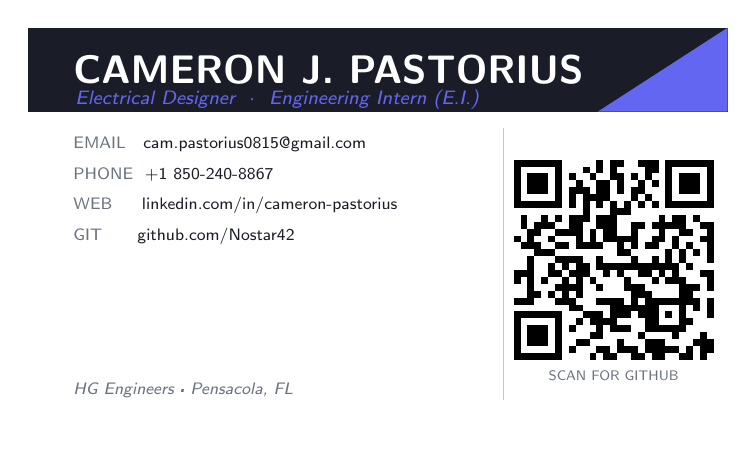
\begin{tikzpicture}[x=1in, y=1in]

  %% Full white background
  \fill[white] (0,0) rectangle (3.5,2);

  %% Dark header bar (top 0.42in)
  \fill[accent] (0, 1.58) rectangle (3.5, 2);

  %% Indigo triangle accent in top-right of header
  \fill[indigo] (2.85,1.58) -- (3.5,1.58) -- (3.5,2) -- cycle;

  %% Name
  \node[anchor=west, text=white,
        font=\fontsize{13.5}{16}\bfseries\sffamily]
    at (0.18, 1.79) {CAMERON J. PASTORIUS};

  %% Title
  \node[anchor=west, text=indigo,
        font=\fontsize{6.8}{8}\itshape\sffamily]
    at (0.19, 1.64) {Electrical Designer \ $\cdot$ \ Engineering Intern (E.I.)};

  %% Vertical divider between contact and QR
  \draw[muted!40, line width=0.4pt] (2.38, 0.14) -- (2.38, 1.50);

  %% Contact block
  \node[anchor=north west, text=accent,
        font=\fontsize{6.2}{11}\sffamily, align=left]
    at (0.18, 1.50) {%
      {\color{muted}EMAIL} \ \ cam.pastorius0815@gmail.com \\
      {\color{muted}PHONE} \ +1\ 850-240-8867 \\
      {\color{muted}WEB} \ \ \ \ linkedin.com/in/cameron-pastorius \\
      {\color{muted}GIT} \ \ \ \ \ github.com/Nostar42
  };

  %% Company bottom-left
  \node[anchor=south west, text=muted,
        font=\fontsize{6}{7}\itshape\sffamily]
    at (0.18, 0.10) {HG Engineers · Pensacola, FL};

  %% QR code right side
  \node[anchor=center] at (2.93, 0.84) {
    \qrcode[height=1.0in, level=M]{https://github.com/Nostar42}
  };

  %% Scan label
  \node[anchor=center, text=muted,
        font=\fontsize{5.5}{7}\sffamily]
    at (2.93, 0.26) {SCAN FOR GITHUB};

\end{tikzpicture}
\end{document}
